\section{Цель работы}
\begin{itemize}
    \item Получение входной характеристики и семейства выходных характеристик биполярного транзистора в схеме с общим эмиттером;
    \item Расчёт усилительного каскада с заданием рабочей точки транзистора с помощью отрицательной обратной связи по току.
\end{itemize}

\section{Исходные данные}
Транзистор - \text{2SC4081UB}, $E_k=10$В.

\section{Рабочее задание}

\subsection{Получение входной характеристики биполярного транзистора}

Соберём схему (см. рис \ref{sch1}).
\begin{figure}[H]
    \centering
    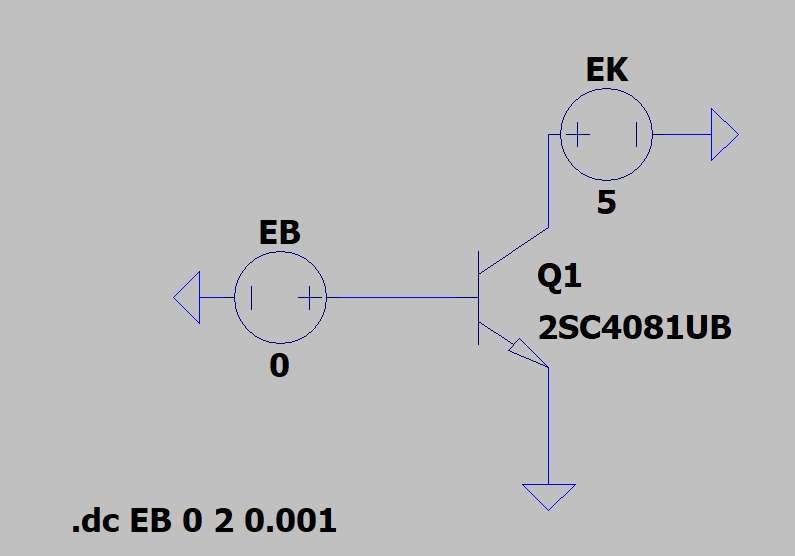
\includegraphics[width=1\linewidth]{Electronics/ELSch_lab2/img/sch1.png}
    \caption{Схема}
    \label{sch1}
\end{figure}
Снимем входную характеристику транзистора (см. рис \ref{o1}).
\begin{figure}[H]
    \centering
    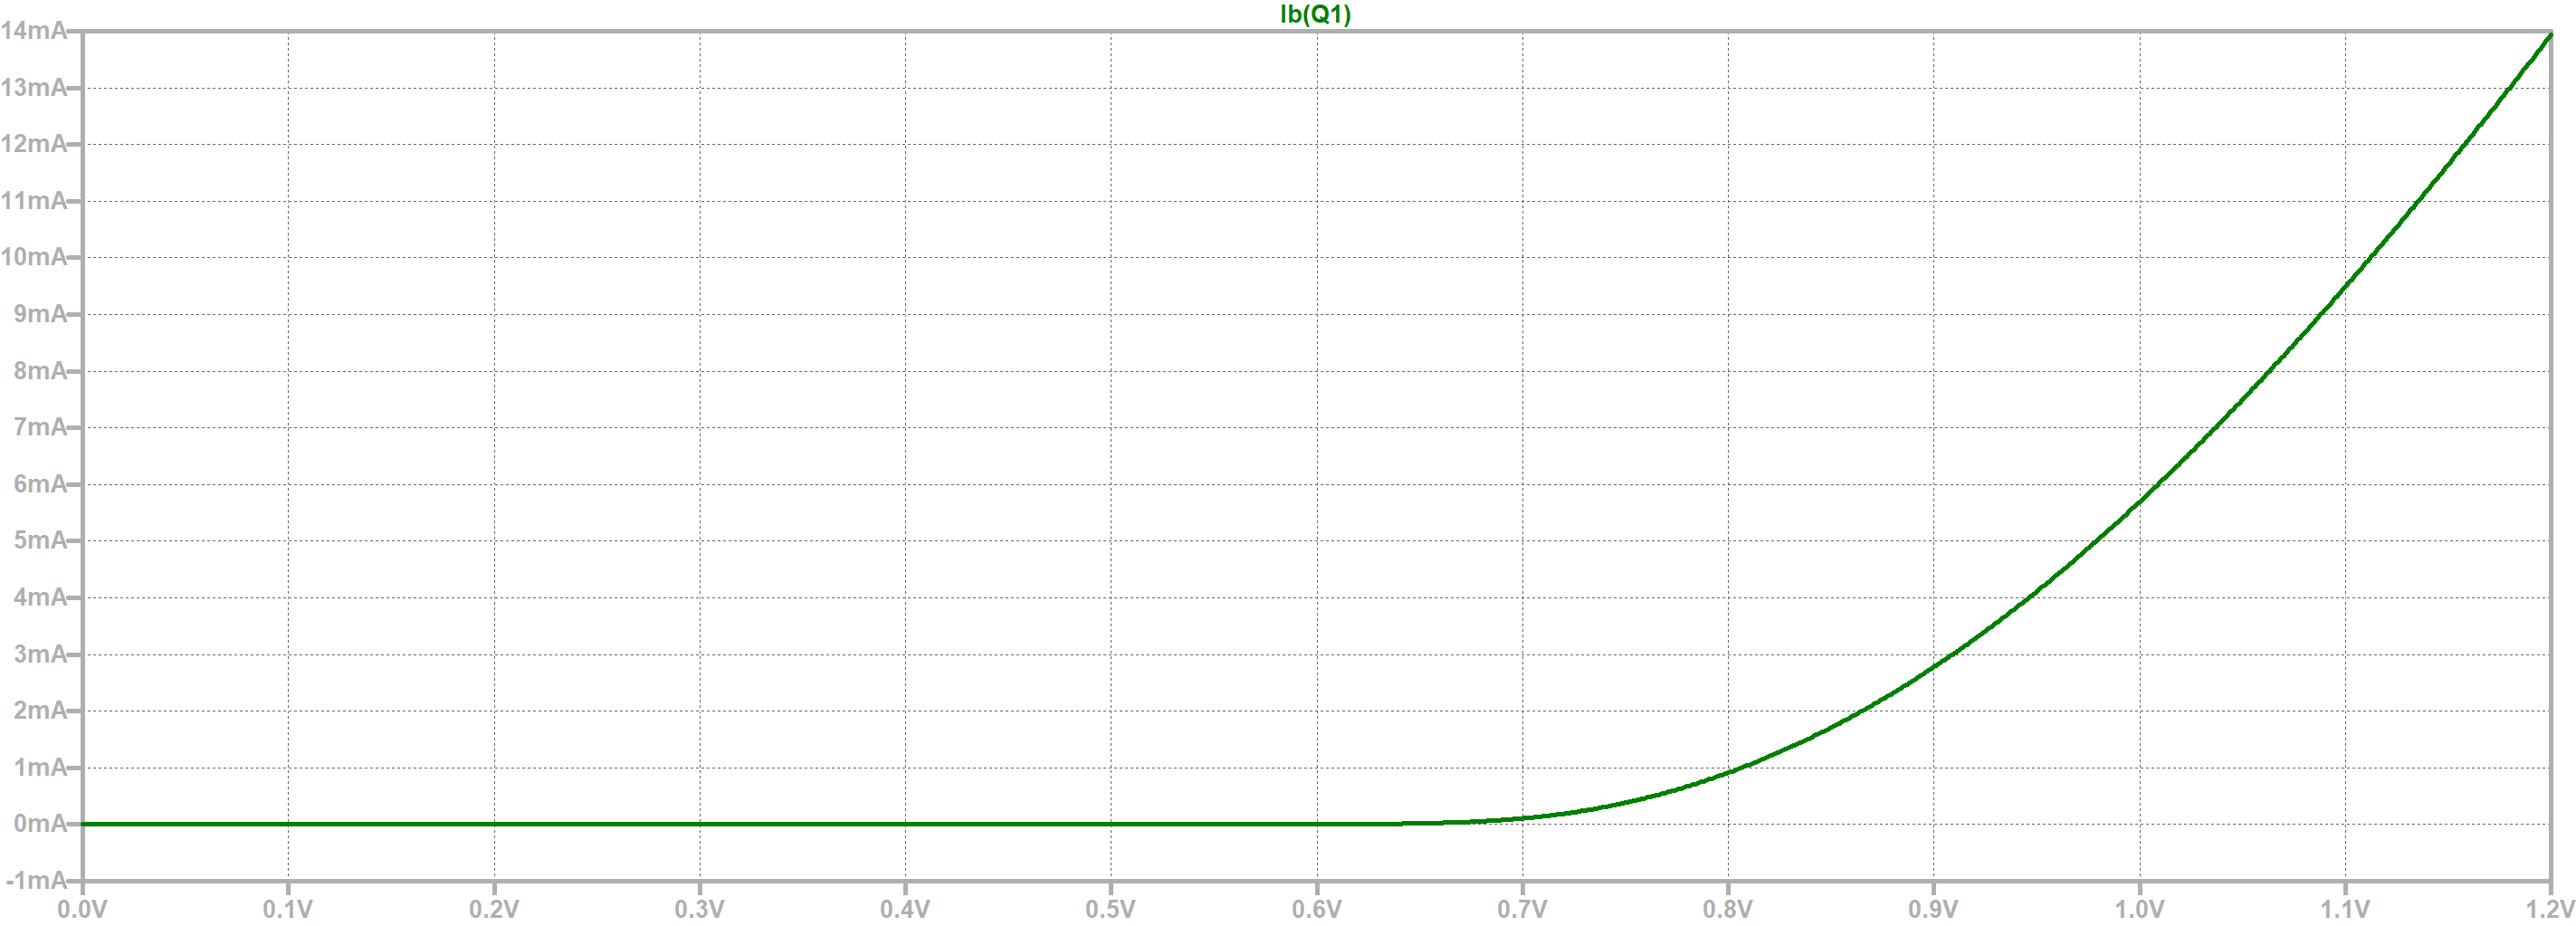
\includegraphics[width=1\linewidth]{Electronics/ELSch_lab2/img/o1.png}
    \caption{ВАХ}
    \label{o1}
\end{figure}

\textbf{Расчёты}\\
Рассчитаем дифференциальное входное сопротивление транзистора: $r_{\text{ВХ}}=\frac{U_{\text{БЭ}}}{I_{\text{Б}}}=\frac{583.0583}{34.131839}=17.08$[Ом].

\subsection{Получение семейства выходных характеристик биполярного транзистора}

Снимем семейство ВАХ при разных токах базы (см. рис \ref{o2}).
\begin{figure}[H]
    \centering
    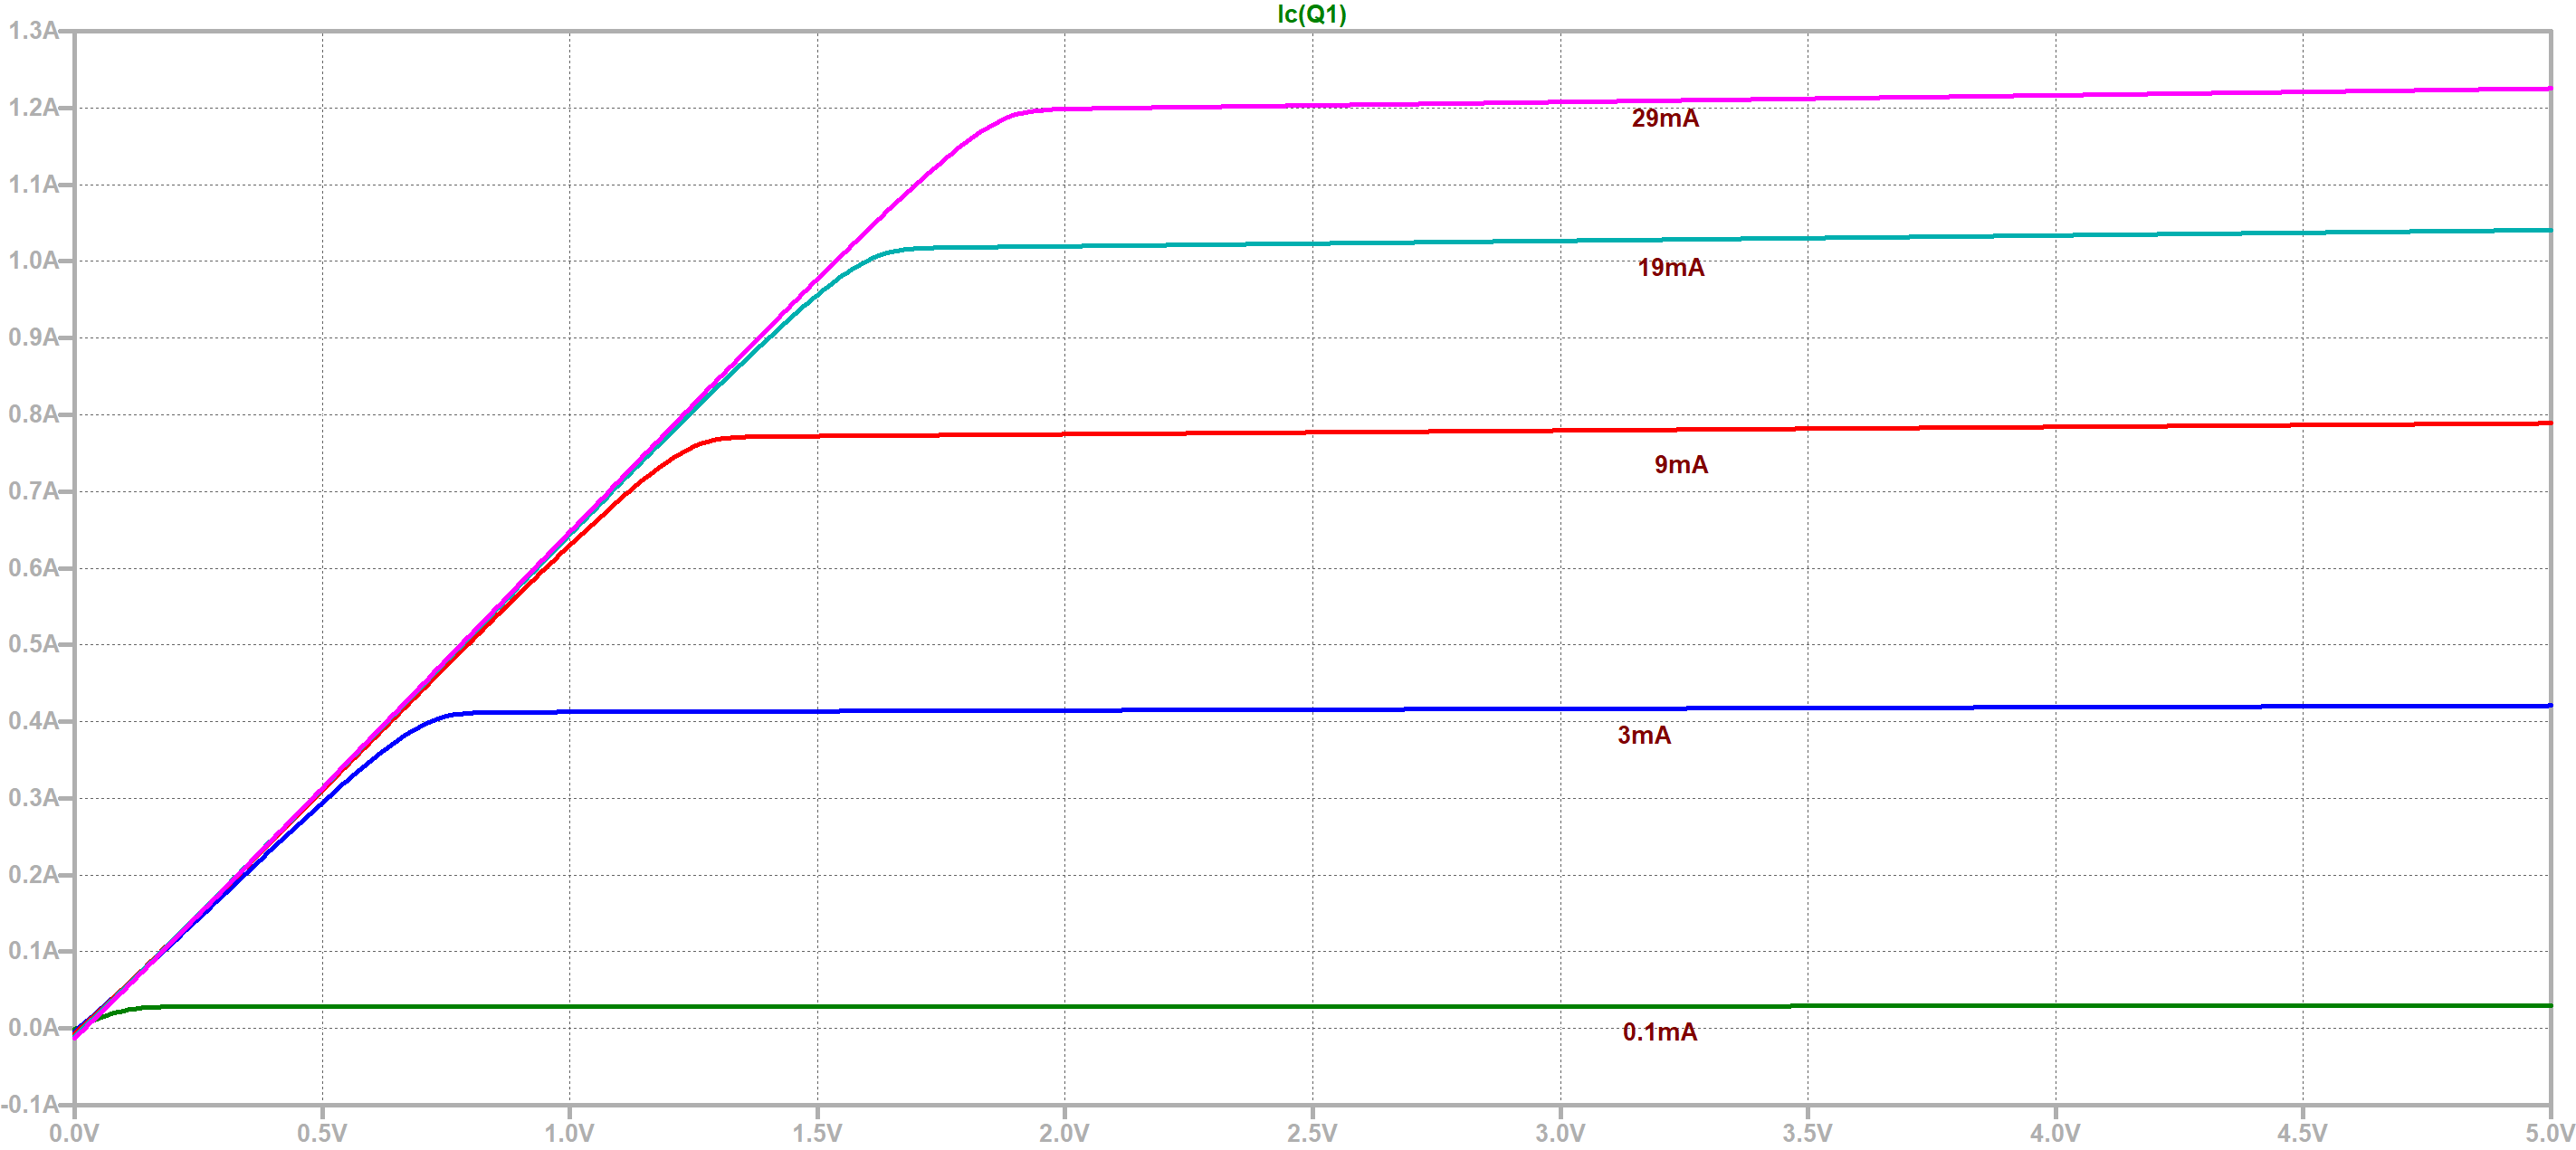
\includegraphics[width=1\linewidth]{Electronics/ELSch_lab2/img/o2.png}
    \caption{ВАХ}
    \label{o2}
\end{figure}

\textbf{Расчёты}\\
Определим значение тока коллектора, соответствующее напряжению коллектор-эмиттер 5 В. Используя полученные значения тока коллектора и значения тока базы, определим коэффициент передачи тока по формуле $\beta_{AC}=\frac{\Delta I_\text{К}}{\Delta I_\text{Б}}$.\\
$\beta_{AC\text{ср}} \approx \frac{18 + 25 + 61,7 + 134,5}{4} \approx 59,8$
\begin{table}[h]
\centering
\large
\begin{tabular}{|c|c|c|}
\hline
\textbf{Ток базы, мА} & \textbf{Ток коллектора, мА} & \textbf{$\beta_{AC}$} \\
\hline
29 & 1220 & --- \\
\hline
19 & 1040 & $\frac{1220-1040}{29-19} = \frac{180}{10} = 18$ \\
\hline
9 & 790 & $\frac{1040-790}{19-9} = \frac{250}{10} = 25$ \\
\hline
3 & 420 & $\frac{790-420}{9-3} = \frac{370}{6} \approx 61,7$ \\
\hline
0,1 & 30 & $\frac{420-30}{3-0,1} = \frac{390}{2,9} \approx 134,5$ \\
\hline
\end{tabular}
\end{table}


\subsection{Задание рабочей точки с помощью отрицательной обратной связи по току}
Определим рабочий диапазон транзистора: $I_{k\_max}=150mA, U_{ke\_max}=50V, P_{max}=200mW$.
Найдем рабочую точку "А" (см. рис. \ref{o3}).
\begin{figure}[H]
    \centering
    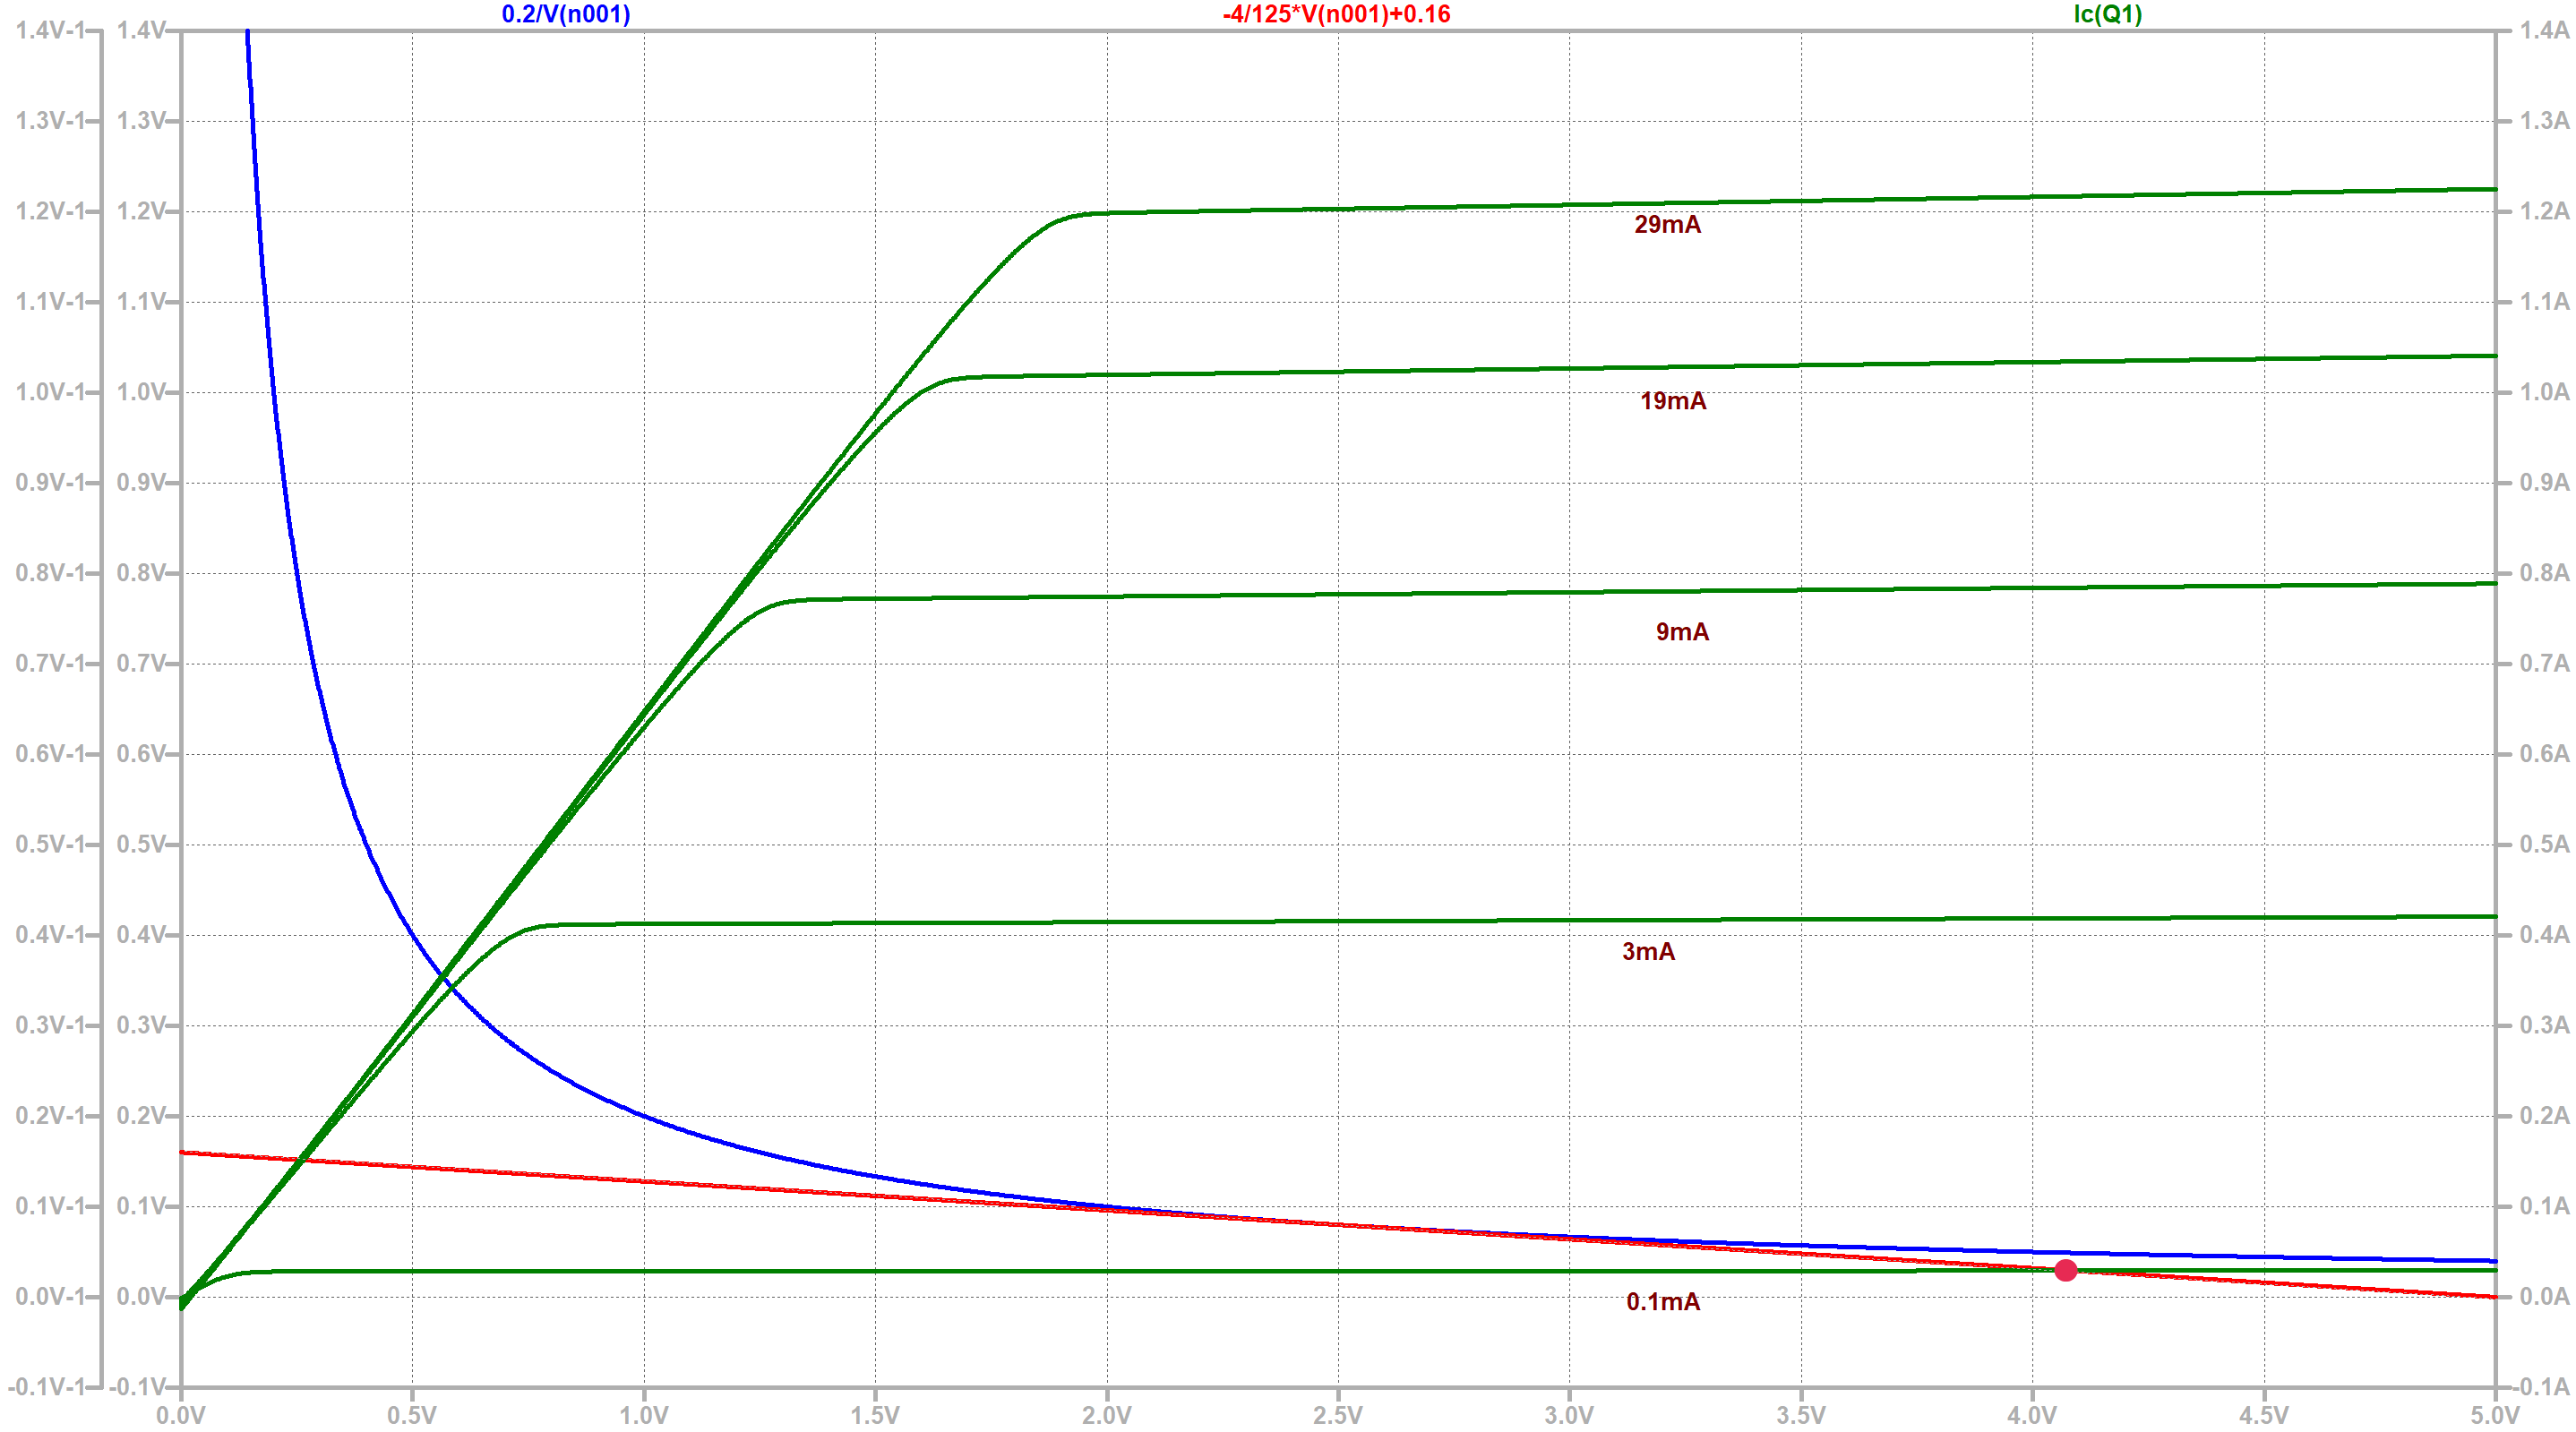
\includegraphics[width=1\linewidth]{Electronics/ELSch_lab2/img/o3.png}
    \caption{Красная точка - рабочая точка}
    \label{o3}
\end{figure}
Координаты точки - $I=29.3mA, U=4.08V$.


\section{Выводы}:



